\subsection{Question 1}

\subsubsection{Point 1}

\begin{equation}
	\begin{aligned}
		f(x) &= \frac{1}{C - x} + x\\
		f(2) &= 1\\
		1 &= \frac{1}{C - 2} + 2\\
		C &= 1
	\end{aligned}
\end{equation}

// TO DO : calcul de stabilité

\subsubsection{Point 2}

\begin{equation}
	\begin{aligned}
		f_2 &= 1\\
		f_{i+1} &= h(1 + (x_i - f_i)^2)+f_i\\
	\end{aligned}
\end{equation}

// TO DO : calcul de h

\subsubsection{Point 3}

\code{littleclasses}{ForwardEuler.java}

Pour adapter le code à une autre fonction, il faut modifier les variables dans la méthode \texttt{main} ainsi que la méthode \texttt{F}. Il est également possible de mettre la fonction exacte dans la méthode \texttt{exactFunction} et de mettre alors le booléen \texttt{compareWithExactFunction} à \texttt{true}. Dans ce cas, le tableau renvoyé par la méthode \texttt{process} contiendra une troisième colonne avec les évaluations pour ces $x$ de la fonction exacte. On peut alors créer un graphe pour comparer les résultats obtenus par Forward Euler et les valeurs exactes avec gnuplot par exemple via la commande suivante :

\begin{lstlisting}
plot 'forward_euler.txt' using 1:2 with lines title 'Forward Euler', '' using 1:3 with lines title 'Exact function'
\end{lstlisting}

\begin{figure}[H]
	\caption{\label{12_forward_1} Forward Euler avec $h=0.25$}
	\centering
	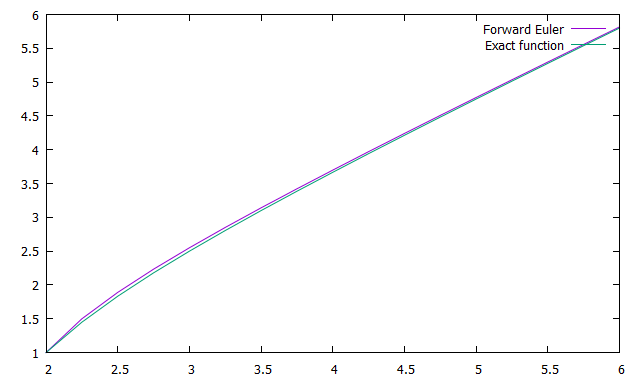
\includegraphics[scale = 0.6]{12_forward_1.png}
\end{figure}


\subsection{Question 2}

\begin{equation}
	\begin{aligned}
	\begin{cases}
	f'(x) = x + \sqrt{f(x)}\\
	f(1) = 2
	\end{cases}
	\end{aligned}
\end{equation}

// TO DO

\subsection{Question 3}

// TO DO

\subsection{Question 4}

// TO DO